\documentclass[oneside,14pt]{extarticle}
\usepackage{cmap}
\usepackage[utf8]{inputenc}
\usepackage[english,ukrainian]{babel}
\usepackage{graphicx}
\usepackage{geometry}
\usepackage{listings}
\usepackage{float}
\usepackage{amsmath}
\usepackage{subfig}
\usepackage{enumitem}
\geometry{
	a4paper,
	left=20mm,
	right=20mm,
	top=15mm,
	bottom=15mm,
}
\lstset{
	language=c,
	tabsize=4,
	keepspaces,
	showstringspaces=false,
	frame=single,
	language=python,
	breaklines=true,
	postbreak=\mbox{{$\hookrightarrow$}\space},
}
\graphicspath{ {./pictures} }
\setlength{\parindent}{4em}

\newcommand\subject{Основи програмування вбудованих систем}
\newcommand\lecturer{професор кафедри ПЗ\\Гавриш В.І.}
\newcommand\teacher{доцент кафедри ПЗ\\Крук О.Г.}
\newcommand\mygroup{ПЗ-32}
\newcommand\lab{3}
\newcommand\theme{Моделювання дискретних $2\pi$- періодичних сигналів
квадратичним поліномом та рядом Фур’є (другий спосіб)}
\newcommand\purpose{Дискретний $2\pi$-періодичний сигнал перетворити в
аналоговий із використанням квадратичного полінома, а після цього
перетворений сигнал наблизити рядом Фур’є}

\begin{document}
\begin{normalsize}
	\begin{titlepage}
		\thispagestyle{empty}
		\begin{center}
			\textbf{МІНІСТЕРСТВО ОСВІТИ І НАУКИ УКРАЇНИ\\
				НАЦІОНАЛЬНИЙ УНІВЕРСИТЕТ "ЛЬВІВСЬКА ПОЛІТЕХНІКА"}
		\end{center}
		\begin{flushright}
			\textbf{ІКНІ}\\
			Кафедра \textbf{ПЗ}
		\end{flushright}
		\vspace{120pt}
		\begin{center}
			\textbf{ЗВІТ}\\
			\vspace{10pt}
			до лабораторної роботи № \lab\\
			\textbf{на тему}: <<\textit{\theme}>>\\
			\textbf{з дисципліни}: <<\subject>>
		\end{center}
		\vspace{40pt}
		\begin{flushright}
			
			\textbf{Лектор}:\\
			\lecturer\\
			\vspace{28pt}
			\textbf{Виконав}:\\
			
			студент групи \mygroup\\
			Коваленко Д.М.\\
			\vspace{28pt}
			\textbf{Прийняв}:\\
			
			\teacher\\
			
			\vspace{28pt}
			«\rule{1cm}{0.15mm}» \rule{1.5cm}{0.15mm} 2024 р.\\
			$\sum$ = \rule{1cm}{0.15mm}……………\\
			
		\end{flushright}
		\vspace{\fill}
		\begin{center}
			\textbf{Львів — 2024}
		\end{center}
	\end{titlepage}
		
	\begin{description}
		\item[Тема.] \theme.
		\item[Мета.] \purpose.
	\end{description}

	\section*{Індивідуальне завдання}
	\begin{enumerate}
		\item Поданий у дискретному вигляді $2\pi$- періодичний сигнал
апроксимувати поліномом другого степеня, коефіцієнти якого визначити за
методом найменших квадратів.
		\item Отриманий перетворений сигнал наблизити рядом Фур’є.
		\item Виконати геометричне зображення дискретного сигналу та кривих,
які описано апроксимаційним квадратичним поліном і рядом Фур’є;
		\item Визначити середні абсолютні похибки, отримані за наближенням
квадратичного полінома та ряду Фур’є.
	\end{enumerate}
	
	\subsection*{Варіант №6}
	
	\begin{equation}
		2,80; 2,94; 3,20; 3,38; 3,53; 3,75\nonumber
	\end{equation}
	
	\section*{Теоретичні відомості}

В цій лабораторній роботі розглядається задача апроксимації дискретних сигналів. Апроксимація сигналів є фундаментальною задачею в області обробки сигналів, що дозволяє представити складний сигнал за допомогою простіших функцій, полегшуючи аналіз та обробку.

\subsection*{Квадратичний поліном}
Квадратичний поліном — це поліном другого степеня, що має загальний вигляд \(y = ax^2 + bx + c\), де \(a\), \(b\), і \(c\) — коефіцієнти полінома. Апроксимація квадратичним поліномом використовується для моделювання тенденцій в даних, коли очікується, що відношення між змінними нелінійне.

\subsection*{Метод найменших квадратів}
Метод найменших квадратів — це стандартний підхід у статистичному моделюванні для знаходження коефіцієнтів апроксимації, мінімізуючи суму квадратів різниць між спостережуваними та апроксимованими значеннями. Цей метод застосовується для визначення коефіцієнтів квадратичного полінома в даній лабораторній роботі.

\subsection*{Ряд Фур'є}
Ряд Фур'є дозволяє представити періодичну функцію через суму синусів і косинусів (або через комплексні експоненти), що мають різні частоти. Коефіцієнти цих тригонометричних функцій знаходять за допомогою інтегралів від добутків функції на відповідні синуси та косинуси. Використання ряду Фур'є дозволяє аналізувати функції у частотному домені.

\subsection*{Аналіз похибок}
Для оцінки якості апроксимації використовуються середня абсолютна похибка (MAE) та середньоквадратична похибка (MSE). Ці метрики дозволяють оцінити відстань між реальними даними та їх апроксимаціями, надаючи кількісну міру точності моделювання.
	
	\section*{Хід роботи}	

	\subsection*{Код програми}
	Файл \textit{main.py}:
	{\small
		\begin{lstlisting}
import numpy as np
import matplotlib.pyplot as plt
from numpy.linalg import lstsq
from numpy.fft import fft, ifft

y = np.array([2.80, 2.94, 3.20, 3.38, 3.53, 3.75])
x = np.linspace(0, 2 * np.pi, len(y), endpoint=False)

A = np.vstack([x**2, x, np.ones(len(x))]).T
coefficients = np.linalg.lstsq(A, y, rcond=None)[0]

poly_approx = A @ coefficients

n = len(y) // 2  # Number of harmonics
c = fft(y) / len(y)  # Fourier coefficients
c[n] = c[n] / 2  # Adjust the middle coefficient if the length is even
fourier_approx = np.real(ifft(c * len(y)))

mae_poly = np.mean(np.abs(y - poly_approx))
mse_poly = np.mean((y - poly_approx)**2)
mae_fourier = np.mean(np.abs(y - fourier_approx))
mse_fourier = np.mean((y - fourier_approx)**2)

plt.figure(figsize=(10, 6))
plt.scatter(x, y, color='red', label='Original Discrete Signal')
plt.plot(x, poly_approx, label='Quadratic Polynomial Approximation', color='blue')
plt.plot(x, fourier_approx, label='Fourier Series Approximation', color='green')
plt.legend()
plt.xlabel('x')
plt.ylabel('Signal Value')
plt.title('Discrete Signal Approximation')
plt.show()

print(f"Quadratic Polynomial Approximation - MAE: {mae_poly:.4f}, MSE: {mse_poly:.4f}")
print(f"Fourier Series Approximation - MAE: {mae_fourier:.4f}, MSE: {mse_fourier:.4f}")\end{lstlisting}
	}
	
	\subsection*{Виконання програми}
	
	\begin{figure}[H]
		\centering
		\vspace{-15pt}
		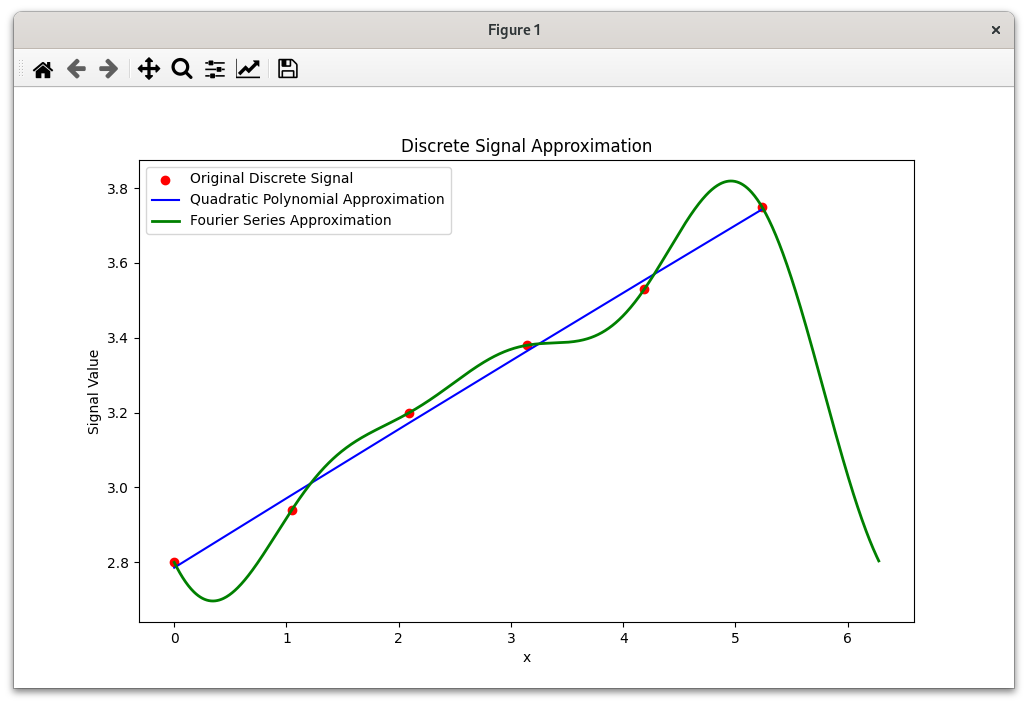
\includegraphics[scale=0.48]{1}
		\vspace{-15pt}
		\caption{Геометричне зображення апроксимації дискретного сигналу апроксимаційним
поліномом та рядом Фур’є.}
	\end{figure}
	
	\begin{table}[H]
		\centering
		\renewcommand{\arraystretch}{1.5}
		\begin{tabular}{|c|c@{\hspace{15pt}}|c@{\hspace{15pt}}|}
			\hline
			Метод & Сер. абс. похибка & Сер. квад. похибка\\ \hline
			Фур'є & 0.045 & 0.002 \\ \hline
			Кв. Поліном & 0.021 & 0.0006 \\ \hline
		\end{tabular}
		\caption{Порівняння середньої абсолютної похибки та середньої квадратичної похибки.}
	\end{table}
	
	\section*{Висновки}
	Під час виконання лабораторної роботи я перетворив дискретний $2\pi$-періодичний сигнал в
аналоговий із використанням квадратичного полінома, а після цього
перетворений сигнал наблизити рядом Фур’є Визначив середню абсолютну похибку
апроксимації та наближення.
	    
\end{normalsize}
\end{document}
